\documentclass{sig-alternate-br}

\bibliographystyle{plain}

\usepackage{placeins}
%\floatbarrier
\usepackage{caption}
\captionsetup{labelfont=bf,font=bf}
\usepackage{subcaption}

\usepackage{listings}
\lstset{	numbers=left,
		escapechar=$,
		breaklines=true,
		numbersep=3pt}


\newtheorem{definition}{Definition}
\newtheorem{lemma}{Lemma}

\title{Proving correctness of Lace using interactive theorem prover tools}
\author{
	\alignauthor
	Thijs van Ede\\
	\affaddr{University of Twente}\\
	\affaddr{P.O. Box 217, 7500AE Enschede}\\
	\affaddr{The Netherlands}\\
	\affaddr{t.s.vanede@student.utwente.nl}\\
}
\date{\today}

\begin{document}
\maketitle

\begin{abstract}
Interactive theorem prover tools 
\end{abstract}

\keywords{interactive theorem prover tool, PVS, Lace, linearisation points, concurrent programming, proof}

\section{Introduction}
Modern day processors' multi-core architecture has increased demand for concurrent programming to fully utilise the processing power.
These concurrent programs need to be proven correct to ensure the desired execution.
Several methods for proving programs correct exist such as separation logic\cite{reynolds2002} and first-order logic\cite{smullyan1995}.

Interactive theorem prover tools such as Isabelle\cite{paulson1994isabelle}, Coq\cite{coq2015}, and PVS\cite{owre1992pvs} use various methods of logical based proving check models.
These tools are helpful in proving properties of both sequential\cite{badban2005verification} and concurrent\cite{colvin2006formal} \cite{shankar1993verification} algorithms.
The theorem prover tool PVS uses several decision procedures and a symbolic model checker, in combination with a random tester to help generating formal proofs.

This paper tries to proof several properties of the Lace algorithm\cite{vanDijk2014206} to illustrate a method of proving concurrent programs.
Lace is a concurrent algorithm for thread scheduling among processors.
Its use of a memory fence, compare-and-swap system call and both concurrent and sequential components make it an ideal algorithm to proof correct.

In this paper, we will prove the Lace algorithm correct using the interactive theorem prover tool PVS.
The algorithm is modeled by constructing linearisation points where the state of the system changes, and using them to generate a flow diagram of the program.
Subsequently, PVS assists in proving the required invariants using this model in combination with several assumptions about the system.
With the invariants a comprehensive proof of the Lace algorithm is constructed.

\subsection{Lace}
Lace is a work stealing algorithm\cite{Blumofe1994} which uses a compare-and-swap operation to steal tasks\cite{vanDijk2014206}.
Each process in Lace has its own deque, i.e. double-ended queue. A deque can be accessed from both its head and its tail, the process itself operates on the head, whereas stealing processes operate on the tail.
Besides the deque, a process also holds pointers for the head and tail of the deque, as well as a pointer for a split point.
This split point indicates whether a thief process can steal a task or not, i.e. what part of the deque is shared and what part is private.
When the tail is still lower than the split point, thief processes are allowed to steal this task.
Conversely, when the tail increases beyond the split point thief processes may not steal the task.
Figure \ref{fig:deq} illustrate the workings of this deque with its head, tail, and split variables.
\begin{figure}[h]
	\centering
	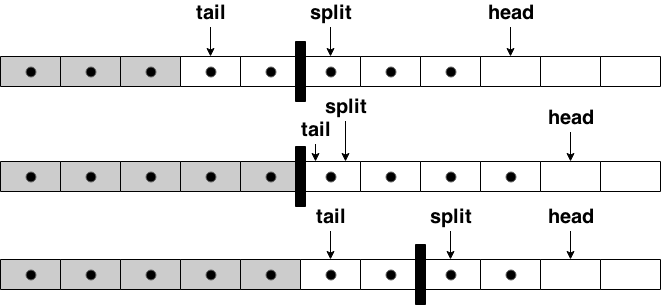
\includegraphics[width=8cm]{Lace_Explanation}
	\caption{Example on manipulation of deque variables.}
	\label{fig:deq}
\end{figure}
The deque is presented as an array of slots which may be empty or contain tasks.
Slots containing a task are represented with a $\bullet$.
We say a task is stolen when it is located left of the tail, i.e. tail points to the next task to be stolen.
The bar before the split point indicates that tasks can only be stolen left of the bar or split point.
In the first deque, tail is still to the left of split, we say $tail < split$, and thus tasks can be stolen.
In the second deque,$ tail = split$ which means thief processes may not steal tasks.
However, in Lace, a thieving process can request to move the split point so more tasks can be stolen.
This grow\_shared request issues the deque process to increase the split point if possible, which is shown in the bottom deque.
When the head wants to execute a task, it will pop it off the head of the deque and point its head pointer to the task before that.
However, if $head = split$ it cannot pop a task, therefore it will try to shrink the shared part of the deque.
If this is possible, i.e. if $tail < split$, split will be moved to the left and head can pop more tasks.
The full algorithm of Lace, as used in the paper can be found in the appendix.

\subsection{PVS}
Concurrent programs such as Lace, can be proven in a variety of different ways.
There exist tools for proving concurrent programs such as VerCors\cite{eemcs24905}, but they give rather little feedback on the workings of the program.
That is, these tools state whether a program works correct, it does not give the reason it works correct.
Since Lace is still being developed, it is desirable to develop understanding of the algorithm.
Interactive theorem prover tools such as PVS are ideally suited for this purpose, since they give feedback on required properties of lemmas and require the user to check whether required properties hold.
PVS in particular comes highly recommended for its abilities to proof concurrent programs\cite{colvin2006formal} \cite{shankar1993verification}.
Therefore, this paper uses PVS as interactive theorem prover tool to prove Lace correct.

\section{Preliminaries}
\subsection{System}
This paper assumes the algorithm runs on a shared memory system with the x86 memory model.
This memory model allows the reordering of loads before stores, that is, write operations are buffered before they are stored in memory.
Thus threads might read old values, even though they have been written by other threads.
These writes may not have become globally visible yet, because they are still buffered.
Memory fences are used to flush these write buffers and make changes globally visible.
Memory stores are immediately visible to threads that wrote them, hence they do not require memory fences.

\subsection{Compare-and-swap}
A compare-and-swap (\texttt{cas}) ensures thread safety by simulating an atomic memory operation.
The \texttt{cas} operation takes three parameters as input, namely a \texttt{variable}, an \texttt{expected value}, and a \texttt{replacement value}.
The \texttt{cas} operation compares the value of \texttt{variable} to the \texttt{expected value}. When those values are equal, the \texttt{replacement value} replaces the current value of \texttt{variable} and \texttt{cas} returns \texttt{true}.
If they are not equal, \texttt{variable} retains its current value and \texttt{cas} returns \texttt{false}.
Because of its atomicity, \texttt{cas} ensures only one thread executes successfully when multiple threads invoke \texttt{cas} with the same valid parameters.
\texttt{cas} is used for concurrent programming as it ensures thread safety and provides feedback to executing threads on whether their operation succeeded or not.

\subsection{Linearisation points}
\label{sec:lin}
An important aspect of proving concurrent algorithms is defining linearisation points\cite{herlihy1990}.
These linearisation points are the points in time the state of the system changes.
When reasoning about concurrent programs, information about the state of the system is needed to predict its expected behaviour.
By defining linearisation points, the order in which they occur can be varied and thereby all possible states can be derived.
That is, by varying the order of linearisation points, all possible equivalent sequential programs can be derived, which in turn can be reasoned about.

\subsection{Assumed properties}
First of all, we have four ways of classifying a task.
\begin{definition}A task x exists $\iff$ x < \texttt{head}\end{definition}
\begin{definition}A task x is stolen $\iff$ x < \texttt{tail}\end{definition}
\begin{definition}A task x is shared $\iff$ x < \texttt{split}\end{definition}
\begin{definition}A task x is private $\iff$ x $\geq$ \texttt{split}\end{definition}
In proving Lace correct, this paper assumes there is only one owner thread per deque and a possibly infinite number of thieving threads.
In practice there are more than one owner threads since there are multiple deques.
However, the proof of correctness for one deque is equivalent to all other deques, i.e. we assume that owner threads are not influenced by each other, only by thieving threads.
The second assumption is that thieving threads only call \texttt{steal} and the owner threads only calls \texttt{push}  and \texttt{pop}.
This implies that the owner thread is also the only thread that has access to \texttt{grow\_shared}  and \texttt{shrink\_shared}, since they are only called in \texttt{push} and \texttt{pop}.
In addition, this paper assumes the number of calls to \texttt{pop} is equal to the number of calls to \texttt{push} when the algorithm finished executing. I.e. the deque is empty when the program finished.
Finally, all deque values - i.e. tail, split, head, and the entries within the deque - are all set to zero when the deque is initialised.
\begin{figure}[h]
	\begin{enumerate}
		\setlength{\itemsep}{-3pt}
		\item One owner thread per deque.
		\item Possibly infinite number of thieving threads per deque.
	
		\item \texttt{steal} is only called by thieving threads.
		\item \texttt{push} and \texttt{pop} are only called by owner thread.
		\item Owner thread only calls \texttt{grow\_shared} and \texttt{shrink\_shared}.
	
		\item Number of \texttt{pop} calls $\leq$ number of \texttt{push} calls.
		\item When finished, number of \texttt{pop} calls = number of \texttt{push} calls.
	
		\item On initialisation all deque variables are set to zero.
	\end{enumerate}
	\caption{Assumed properties of Lace}
\end{figure}

\subsection{Required properties}
Lace requires some properties to work correctly.
First of all, the variables \texttt{head}, \texttt{split}, and \texttt{tail} should stay within bounds.
Figure \ref{inv:bounds} expresses this requirement as invariants. 
\begin{figure}[h]
	\texttt{0 $\leq$ head $\leq$ size}\\
	\texttt{0 $\leq$ split $\leq$ head}\\
	\texttt{0 $\leq$ tail $\leq$ head}
	\caption{Invariants: variables stay within bounds.}
	\label{inv:bounds}
\end{figure}
Furthermore, a task must be stolen only once, and executed exactly once.
To prove these properties, they are written as invariants.
When every task is stolen only once, it means thieving threads can only steal tasks $\geq$ \texttt{tail} and that when tail reduces, a task cannot be stolen again. The former part of the property is trivial, if tail increases it steals an unstolen task which is consistent with the requirement. The latter part is less trivial, if tail reduces, a stolen task cannot be executed again, therefore the stolen tasks need to be removed before tail is reduced. This is written as an invariant in Figure \ref{inv:stolen}.
\begin{figure}[h]
	\texttt{tail.new > tail.old || (tail.new $\leq$ tail.old \&\& tail.old == head \&\& pop() == STOLEN, head)}
	\caption{Invariant: every task is stolen only once.}
	\label{inv:stolen}
\end{figure}
To elaborate on this invariant: either \texttt{tail} increases when a new task is stolen, or \texttt{tail} decreases but the task has to be removed from the deque so that it cannot be stolen again.
When a task is executed once, this implies it is only stolen once and not executed by the owner thread, or it is executed by the owner thread and never stolen. This can be written as the invariant in Figure \ref{inv:exec}.
\begin{figure}[h]
	\texttt{(pop() == STOLEN \&\& head.new < head.old) || (pop() == WORK \&\& head.new < head.old)}
	\caption{Invariant: every task is executed only once.}
	\label{inv:exec}
\end{figure}

\section{Method}
In proving concurrent programs such as Lace using interactive theorem prover tools, linearisation points of the algorithm must be appointed.
Each linearisation point modifies a variable of the program.
For concurrent programs, each possible state of the system can be derived by altering the order in which the linearisation points occur.
From which conclusions can be drawn about the desired behaviour of the system with respect to the possible behaviour of the system.

The first step of appointing linearisation points is trivial and could be done automatically.
However, because the algorithm is relatively simple and to illustrate how these points can be identified it is done manually.
First all global variables of the algorithm are identified, then each point in the algorithm where a variable is changed is appointed as a linearisation point with the operation that is performed at that point.
This is done for all global variables, i.e. \texttt{head, split, tail, allstolen, movesplit} as well as private variables \texttt{o\_allstolen} and \texttt{o\_split}.

After the linearisation points are established, this paper deduces the order in which they occur.
Therefore, we setup flow diagrams of the methods \texttt{pop} and \texttt{push} to establish the possible orders of linearisation points.
These diagrams include methods invoked within the \texttt{pop} or \texttt{push} method.
No flow diagram is setup for the method \texttt{steal}, since we assume numerous threads execute this method simultaneously which renders a diagram useless.

Finally, we prove the required properties of Lace using several lemmas which base themselves on the linearisation points of the system and the possible order of these points.
For these proofs, the interactive theorem prover tool PVS\cite{owre1992pvs} is used which correctly states whether lemmas hold.
These lemmas, as well as axioms are introduces by the user into PVS.
Within this paper, all lemmas and axioms are deduced from the assumptions about Lace, constructed linearisation points, and their order as described by the flow diagrams.
In this paper, PVS' grind option\cite{PVSProverGuide} is used extensively to proof lemmas within the theorem prover tool.
This option attempts to solve given lemmas automatically using lemmas introduces by the user.
Ultimately, the invariant \texttt{(pop() == STOLEN \&\& head.new < head.old) || (pop() == WORK \&\& head.new < head.old)} is proven which establishes correctness of Lace.

Various interactive theorem prover tools may be used for proving this algorithm correct.
However, this paper uses the PVS 6.0 Allegro Lisp Binary for a Linux Intell 64-bit machine.
The model of the algorithm is constructed from its description in the paper \cite{vanDijk2014206}.

A proof constructed with an interactive theorem prover such as PVS holds in all cases and could also be constructed without using PVS.
The tool only helps to construct the proof and formalise the method of proving algorithms correct.
Therefore, PVS speeds up the process of constructing a proof and increasing confidence in that proof.
It also increases the transferability of this research since the tool constructs equal proofs in an identical way.

\section{Modeling Lace}
A model for the Lace algorithm is constructed from its specifications as described in \cite{vanDijk2014206} and displayed in Figure \ref{fig:Lace}.
Note the that Figure \ref{fig:Lace} projects a slightly different form of the algorithm.
However, this alternate form is used to construct a model for Lace.
First of all, a model is created from the algorithm without the \texttt{allstolen} flag.

\subsection{Linearisation Points}
In Lace, the state of the system depends on variables head, split, and tail.
The linearisation points are defined on these variables and can be found in Table \ref{tab:head}, \ref{tab:split}, and \ref{tab:tail} respectively.
Note that the variables used at linearisation points to change the state of the system are read at a point before they are used.
Thus the value might have changed when the program reaches the linearisation point, in which case it still uses the old value.
In addition to these three main variables, the algorithm also uses a \texttt{movesplit} and \texttt{allstolen} variable.
These variables influence the behaviour of the system by indicating whether the split point must be moved or all public tasks are stolen respectively.
Therefore, these variables are also included in the linearisation points, which can be found in Table \ref{tab:move}, \ref{tab:allst}, and \ref{tab:oallst}.

\subsubsection{Head}
\label{sec:head}
Variable head is modified in both \texttt{push} and \texttt{pop} methods.
Table \ref{tab:head} gives an overview of the linearisation points and the places where the variables used in the linearisation points are initialised.
The first linearisation point is at line 13 of Lace as shown in Figure \ref{fig:Lace}, where \texttt{head} is incremented by 1.
In this case the variable \texttt{head} is read in the same line of code but does not occur simultaneously with the write operation.
The second and third linearisation points are at line 45 and 47 of Lace as shown in Figure \ref{fig:Lace} respectively.
In both cases, \texttt{head} is decreased by 1 and the variable is read in the same line of code as it is written.
As with the first point, the read and write operation do not occur simultaneously.

\subsubsection{Split}
In Lace, the variable \texttt{split} has two instances, namely \texttt{split} and \texttt{o\_split}.
The latter instance of \texttt{split} is private, and thus visible to the owner thread but not to thieving threads.
To avoid confusion, \texttt{split} and \texttt{o\_split} are displayed in Table \ref{tab:split} and Table \ref{tab:osplit} respectively.
Just as explained in section \ref{sec:head} these tables indicate the methods, linearisation points, operations, initialisation points, and variables for the variable scrutinised, in this case the \texttt{split} and \texttt{o\_split} variables.
As opposed to the linearisation points of the variable \texttt{head}, \texttt{split} has linearisation points in which variables are used that are read in a different line of the algorithm.
This might indicate a greater chance of the variables being altered before they are used.

\subsubsection{Tail}
The final variable of the deque that is important to include in the model is \texttt{tail}, its linearisation points can be found in Table \ref{tab:tail}.
This variable is modified in the \texttt{steal} and \texttt{push} functions at lines 5 and 15 respectively.
In \texttt{steal, tail} is read at line 3 whilst incremented at line 5.
Because of this gap tail can be modified in the meantime by other threads.
The same goes for the modification of \texttt{tail} in \texttt{push}, since read and write do not occur simultaneously.

\subsubsection{Movesplit}
\texttt{movesplit} is not part of the deque, but it indicates whether the owner thread should grow the shared part of the deque.
This boolean variable is set to true at line 8 of the algorithm and is set to false at lines 16 and 25.
These linearisation points can be found in Table \ref{tab:move}.

\subsubsection{Allstolen}
As with \texttt{split}, the variable \texttt{allstolen} has two instances, namely \texttt{allstolen} and \texttt{o\_allstolen}.
The global boolean variable \texttt{allstolen} is set to false at line 17 of the algorithm and to true at line 39.
The private \texttt{o\_allstolen} is set to false and true at lines 19 and 40 respectively.
The linearisation points can be found in Table \ref{tab:allst} and \ref{tab:oallst}.
\begin{table}[h]
	\begin{subtable}[h]{0.45\textwidth}
		\centering
		\begin{tabular}{|l|l|l|l|}
			\hline
			\textbf{method} & \textbf{lin pt} & \textbf{new value} & \textbf{init point} \\ \hline
			push            & 13                 & head+1      & 13               \\ \hline
			pop             & 45                 & head-1      & 45               \\ \hline
			pop             & 47                 & head-1      & 47               \\ \hline
		\end{tabular}
		\caption{Linearisation points of head variable.}
		\label{tab:head}
	\end{subtable}
	\hfill
	\begin{subtable}[h]{0.45\textwidth}
		\centering
		\begin{tabular}{|l|l|l|l|}
			\hline
			\textbf{method} & \textbf{lin pt} & \textbf{new value} & \textbf{init point} \\ \hline
			push            & 15                 & head        		   & 15\\ \hline
			gr\_shared    & 23                 & new\_s=(o+h+1)/2 & 22\\ \hline
			shr\_shared  & 30                 & new\_s=(t+s)/2      & 27\\ \hline
			shr\_shared  & 36                 & new\_s=(t+s)/2      & t:32,s:27\\ \hline
		\end{tabular}
		\caption{Linearisation points of split variable.}
		\label{tab:split}
	\end{subtable}
	\hfill
	\begin{subtable}[h]{0.45\textwidth}
		\centering
		\begin{tabular}{|l|l|l|l|}
			\hline
			\textbf{method} & \textbf{lin pt} & \textbf{new value} & \textbf{init point}\\ \hline
			push            & 18                 & head        & 18\\ \hline
			gr\_shared    & 24                 & new\_s=(o+h+1)/2      & 22\\ \hline
			shr\_shared  & 37                 & new\_s=(t+s)/2      & 27\\ \hline
			shr\_shared  & 37                 & new\_s=(t+s)/2      & t:32,s:27\\ \hline
		\end{tabular}
		\caption{Linearisation points of o\_split variable.}
		\label{tab:osplit}
	\end{subtable}
	\hfill
	\begin{subtable}[h]{0.45\textwidth}
		\centering
		\begin{tabular}{|l|l|l|l|}
			\hline
			\textbf{method} & \textbf{lin point} & \textbf{new value} & \textbf{init point}\\ \hline
			steal           & 5                  & t+1         & 3\\ \hline
			push            & 15                 & head-1      & 15\\ \hline
		\end{tabular}
		\caption{Linearisation points of tail variable}
		\label{tab:tail}
	\end{subtable}
	\begin{subtable}[h]{0.45\textwidth}
		\centering
		\begin{tabular}{|l|l|l|l|}
			\hline
			\textbf{method} & \textbf{lin point} & \textbf{new value} & \textbf{init point}\\ \hline
			steal           & 8                  & true        & 8                   \\ \hline
			push            & 16                 & false       & 16                  \\ \hline
			grow\_shared    & 25                 & false       & 25             \\ \hline
		\end{tabular}
		\caption{Linearisation points of movesplit variable}
		\label{tab:move}
	\end{subtable}
	\begin{subtable}[h]{0.45\textwidth}
		\centering
		\begin{tabular}{|l|l|l|l|}
			\hline
			\textbf{method} & \textbf{lin point} & \textbf{new value} & \textbf{init point}\\ \hline
			push            & 17                 & false       & 17                  \\ \hline
			shrink\_shared  & 39                 & true        & 39               \\ \hline
		\end{tabular}
		\caption{Linearisation points of allstolen variable}
		\label{tab:allst}
	\end{subtable}
	\begin{subtable}[h]{0.45\textwidth}
		\centering
		\begin{tabular}{|l|l|l|l|}
			\hline
			\textbf{method} & \textbf{lin point} & \textbf{new value} & \textbf{init point} \\ \hline
			push            & 19                 & false       & 19                 \\ \hline
			shrink\_shared  & 40                 & true        & 40            \\ \hline
		\end{tabular}
		\caption{Linearisation points of o\_allstolen variable}
		\label{tab:oallst}
	\end{subtable}
	\caption{The method column indicates the method where the variable is modified. Lin pt column refers to the linearisation point in the Lace algorithm as shown in Figure \ref{fig:Lace}. The op column explains the executed operation. The final column init point refers to the point in the Lace algorithm where the variables are read. Note that in \ref{tab:split} and \ref{tab:osplit} o\_split and head are abbreviated to o, h respectively. Tail and split are abbreviated to t and s since these is a local variables as in the algorithm.}
\end{table}

\subsection{Order of linearisation points}
By assuming only one owner thread exclusively calls methods \texttt{push} and \texttt{pop}, all variables manipulated only at those methods will occur in order.
Subsequently, this is true for all methods \texttt{grow\_shared} and \texttt{shrink\_shared} which are invoked only through \texttt{push} and \texttt{pop}.
The natural order of linearisation points called by \texttt{push} and \texttt{pop} can be derived by creating a flow diagram.
In this section, the order of linearisation points for \texttt{push} and \texttt{pop} are derived respectively.

First of all, the method \texttt{push} has a flow diagram as depicted in Figure \ref{fig:push}.
Here the first linearisation point is at line 13, where head is increased.
If \texttt{o\_allstolen} is set, the program continues with linearisation point 15.
Then, if \texttt{movesplit} is true, it is set to false, otherwise it continues flowing through all linearisation points down to linearisation point 19 where \texttt{o\_allstolen} is set to false.
Alternatively, when \texttt{o\_allstolen} is false at line 14 and \texttt{movesplit} is true at line 20, it invokes the method \texttt{grow\_shared} which is depicted as the right part of the flow diagram.
\begin{figure}[h]
	\centering
	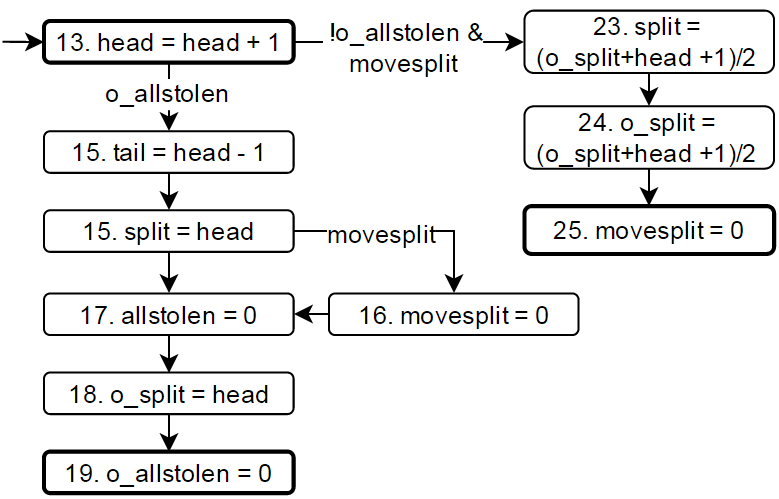
\includegraphics[scale=0.35]{Push_flow_diagram_2.png}
	\caption{Flow diagram of method push.}
	\label{fig:push}
\end{figure}

Second, the method \texttt{pop} has a flow diagram as depicted in Figure \ref{fig:pop}.
This diagram is less trivial than the \texttt{push} flow diagram.
Since the method \texttt{pop} first checks whether \texttt{head} equals 0 and returns when it does, the linearisation points are not reached, thus the first condition of \texttt{head $\neq$ 0} is introduced.
After this, it checks whether \texttt{o\_allstolen} is set, if this is the case, it continues to decrease \texttt{head} and returns.
Alternatively, if \texttt{o\_allstolen} is \texttt{false}, it checks whether \texttt{o\_split == head}, if so, it calls the method \texttt{shrink\_shared} following the rhombus' upper arrow.
The method \texttt{shrink\_shared} first checks whether the variables \texttt{t} and \texttt{s} that it read from \texttt{tail} and \texttt{split} respectively are equal.
If this condition is true, it sets \texttt{allstolen} and \texttt{o\_allstolen} after which it returns true and continues at \texttt{pop}.
Subsequently, if the condition is false, it modifies \texttt{split} and sets a memory fence, depicted with the dashed lines.
After reading the \texttt{tail} variable into \texttt{t} again, the algorithm checks whether \texttt{t} equals \texttt{s}.
When they are equal, the method sets the \texttt{allstolen} variables, and returns true, after which it continues at \texttt{pop}.
However, when they are not equal, \texttt{t} and the temporary variable \texttt{new\_s} are compared.
If \texttt{t $>$ new\_s}, \texttt{split} is modified, otherwise only \texttt{o\_split} is set to \texttt{new\_s}.
Thereafter, the method returns false and continues at \texttt{pop}.
\begin{figure}[h]
	\centering
	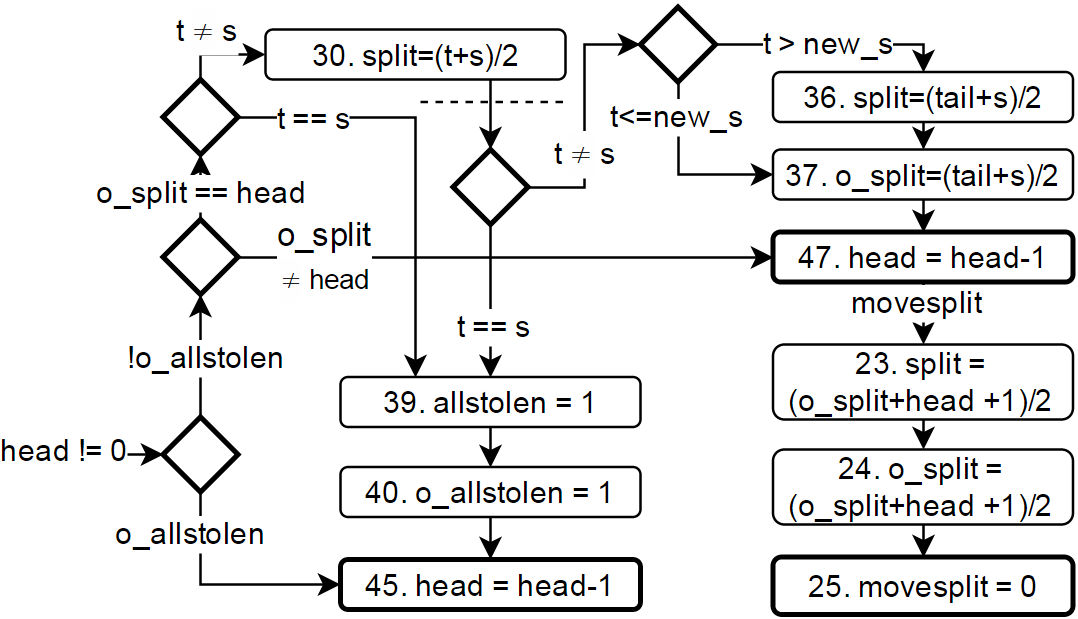
\includegraphics[scale=0.25]{Pop_flow_diagram_2.png}
	\caption{Flow diagram of method pop.}
	\label{fig:pop}
\end{figure}

From these flow diagrams, the possible sequences of linearisation points are clear.
Note that the linearisation points modified by thieving threads through the method \texttt{steal} are not included.
Since these occur at arbitrary points in the algorithm, it does not make sense to include them in a flow chart.

\section{Proving Lace}
%%%%%%%%%%%%%%%%%%%%%%%%%%%%%%%%%
%				allstolen = o_allstolen					%
%%%%%%%%%%%%%%%%%%%%%%%%%%%%%%%%%
\begin{lemma}
	\texttt{allstolen = o\_allstolen} at load operations.
	\label{lem:allstolen}
\end{lemma}
\begin{proof}
	Table \ref{tab:allst} and \ref{tab:oallst} indicate that both \texttt{allstolen} variables only change through methods \texttt{push} and \texttt{shrink\_\\shared}.
	Figure \ref{fig:push} states that private variable \texttt{o\_split} is the only variable to change in between the modifications to \texttt{false} of the \texttt{allstolen} variables.
	Subsequently, Figure \ref{fig:pop} states there are no linearisation between the modifications to \texttt{true} at all.
	No load operations of \texttt{allstolen} or \texttt{o\_allstolen} occur in between either modification of the variables.
	The assumed memory model where loads can be reordered before stores does not influence this Lemma, since Table \ref{tab:allst} states stealing threads only use \texttt{allstolen}.
	The owner thread does not reorder both \texttt{allstolen} variables, because the thread itself is the only thread modifying them.
\end{proof}

%%%%%%%%%%%%%%%%%%%%%%%%%%%%%%%%%
%					split = o_split					%
%%%%%%%%%%%%%%%%%%%%%%%%%%%%%%%%%
\begin{lemma}
	\texttt{split = o\_split} at load operations.
	\label{lem:split}
\end{lemma}
\begin{proof}
	Table \ref{tab:split} and \ref{tab:osplit} affirm that both \texttt{split} variables only change through methods \texttt{push}, \texttt{grow\_shared}, and \texttt{shrink\_shared}.
	Figure \ref{fig:push} indicates that private variable \texttt{movesplit} and \texttt{allstolen} are modified between the linearisation points of the \texttt{split} variables.
	Furthermore, Figure \ref{fig:pop} states that between linearisation points 23 and 24 no reads of either split variable occur.
	Between linearisation point 30 of \texttt{split} and 37 of \texttt{o\_split} there are no read operations for either \texttt{split} variable.
	In addition, between linearisation point 36 of \texttt{split} and linearisation point 37 of \texttt{o\_split} there are no read operations on \texttt{split}.	
	The x86 memory model where loads can be reordered before stores is not important for this Lemma, since the method \texttt{steal} only uses \texttt{split}.
	Whereas the owner thread uses \texttt{o\_split}, but loads cannot be reordered before stores for the thread that executes the stores.		
\end{proof}

%%%%%%%%%%%%%%%%%%%%%%%%%%%%%%%%%
%				    0 <= head < size					%
%%%%%%%%%%%%%%%%%%%%%%%%%%%%%%%%%
\begin{lemma}
	\texttt{0 $\leq$ head $\leq$ size}.
	\label{lem:headsize}
\end{lemma}
\begin{proof}
	Table \ref{tab:head} indicates \texttt{head} is only increased at method \texttt{push} and decreased at the method \texttt{pop}.
	This indicates there is no need to take the reordering of loads before stores into account, since only one thread operates on this variable.
	Since we assume \texttt{head} = 0 at the start of the algorithm, i.e. \texttt{0 $\leq$ head < size}, it is left to prove linearisation point 13 cannot increase \texttt{head} beyond \texttt{size}.
	Subsequently, we prove linearisation points 45 and 47 cannot decrease \texttt{head} to a value lower than 0.
	In PVS we input the code as depicted in Figure \ref{pvs:head}.
	To proof lemma \texttt{lemma\_size}, we use axioms \texttt{head\_start}, stating \texttt{head} < \texttt{size} at the initialisation, and \texttt{head\_size} stating \texttt{head $\neq$ size}, i.e. line 11 of Lace.
	Then, we expand function \texttt{incr\_head(head)}, which increases \texttt{head} by 1, i.e. line 13 of Lace.
	Then using PVS' grind option, it concludes that indeed the lemma holds.
	Proving \texttt{head} cannot decrease to a value lower than 0, we use axioms \texttt{head\_start} and \texttt{head\_zero} and prove \texttt{lemma\_zero} using PVS' grind option.
	This concludes that the lemma holds.
\end{proof}
\begin{figure}[h]
	\texttt{head\_start: AXIOM head >= 0 AND head < size}\\
	\texttt{head\_zero:  AXIOM NOT (head = 0)}\\
	\texttt{head\_size:  AXIOM NOT (head = size)}\\\\
	\texttt{incr\_head(head): posnat = head+1}\\
	\texttt{decr\_head(head): posnat = head-1}\\\\
	\texttt{lemma\_size: LEMMA incr\_head(head) <= size}
	\texttt{lemma\_zero: LEMMA decr\_head(head) >= 0}
	\caption{PVS proof of 0 $\leq$ head $\leq$ size}
	\label{pvs:head}
\end{figure}

%%%%%%%%%%%%%%%%%%%%%%%%%%%%%%%%%
%		  tail+1 ==> !allstolen && t=tail < s=split 			%
%%%%%%%%%%%%%%%%%%%%%%%%%%%%%%%%%
\begin{lemma}
	\texttt{tail.new = tail.old+1 $\Rightarrow$ !allstolen} and \texttt{t < s} and \texttt{t == tail} and \texttt{s == split}
	\label{lem:incrtail}
\end{lemma}
\begin{proof}
	The only linearisation point where \texttt{tail} is increased is at the \texttt{cas} operation of line 5 as stated in Table \ref{tab:tail}. This modification only succeeds if \texttt{cas} succeeds, i.e. if the compare-and-swap method returns true. Thus this can be modeled in PVS as described in Figure \ref{pvs:tailincr}.
\end{proof}
\begin{figure}[h]
	\texttt{cas(var1, var2, exp1, exp2, val1, val2: posnat) : bool = IF (var1 = exp1 AND var2 = exp2 THEN true ELSE false ENDIF}\\\\
	\texttt{steal(t, s, tail, split, allstolen): bool = IF allstolen THEN false ELSE (IF t < s THEN cas(t,s,tail,split,(t+1),s) ELSE false ENDIF) ENDIF}\\\\
	\texttt{lem\_incr\_tail: LEMMA (NOT allstolen AND t < s AND t = tail AND s = split) IMPLIES steal(t,s,tail,split,allstolen) = true}\\
	\texttt{lem\_incr\_tail: LEMMA NOT (NOT allstolen AND t < s AND t = tail AND s = split) IMPLIES steal(t,s,tail,split,allstolen) = false}
	\caption{PVS proof of incrementing tail}
	\label{pvs:tailincr}
\end{figure}

%%%%%%%%%%%%%%%%%%%%%%%%%%%%%%%%%
%	      Linearisation point 30 => split.new <= split.old 	 	%
%%%%%%%%%%%%%%%%%%%%%%%%%%%%%%%%%
\begin{lemma}
	Linearisation point 30 $\Rightarrow$ \texttt{split.new $\leq$\\ split.old}
	\label{lem:lin30}
\end{lemma}
\begin{proof}
	Lemma \texttt{lem\_decr\_a} in Figure \ref{pvs:decrtail} corresponds to line 30 of Lace and states that \texttt{decr\_tail} $\leq$ \texttt{split}, under the assumptions that \texttt{tail != split} and \texttt{tail < split}.
	The former assumption is valid since Figure \ref{fig:pop} states the variables \texttt{tail} and \texttt{split} are not equal when linearisation point 30 occurs and the read variables \texttt{tail} and \texttt{split} are not modified in between.
	The latter assumption is valid since Lemma \ref{lem:incrtail} states \texttt{tail} cannot increase if \texttt{tail $\geq$ split} and at the start of Lace \texttt{tail == split == 0}.
	Using PVS' grind option, this Lemma is proven correct.
\end{proof}

%%%%%%%%%%%%%%%%%%%%%%%%%%%%%%%%%
%	      Linearisation point 36 => split.new <= split.old 	 	%
%%%%%%%%%%%%%%%%%%%%%%%%%%%%%%%%%
\begin{lemma}
	Linearisation point 36 $\Rightarrow$ \texttt{split.new $\leq$ \\split.old} where \texttt{split.old} is before Linearisation point 30. 
	\label{lem:lin36}
\end{lemma}
\begin{proof}
	Lemma \texttt{lem\_decr\_b} in Figure \ref{pvs:decrtail} corresponds to the linearisation point of line 36 of Lace and states that after the linearsation point of line 30, line 36 can increase \texttt{split}, but not beyond the point of \texttt{split.old}, i.e. \texttt{split} before the linearisation point of line 30.
	It assumes \texttt{tail != split} and \texttt{t > decr\_tail(tail,split)} and \texttt{t < split}.
	The first of these assumptions is true according to Figure \ref{fig:pop}, it shows \texttt{t != s} is a requirement for reaching linearisation point 36.
	Since \texttt{tail} is reread at line 32, but \texttt{split} is equal to the value read at line 27 this assumption still holds.
	The second assumption is valid since Figure \ref{fig:pop} expounds \texttt{t > new\_s} for linearisation point 36 to be reached.
	That is, the newly read value of \texttt{tail} here modeled as \texttt{t} is larger than the computed value of \texttt{split} at linearisation point 30.
	Note that the newly read value of \texttt{tail} cannot increase any further, since the memory fence of line 31 asserts the modification of \texttt{split} is globally visible.
	Any reordering of read and write operations as the x86 memory model allow do not apply in this part of the code since the memory fence forces global visibility.
	The final assumption of \texttt{t < split} is true since Lemma \ref{lem:incrtail} affirms \texttt{tail} cannot increase unless it is smaller than \texttt{split}.
	With these assumptions, PVS shows that indeed the newly computed value of \texttt{split.new $\leq$ split.old}.
\end{proof}

%%%%%%%%%%%%%%%%%%%%%%%%%%%%%%%%%
%			Global visibility min(lin 30, lin 36)			 	%
%%%%%%%%%%%%%%%%%%%%%%%%%%%%%%%%%
\begin{lemma}
	\texttt{min(linearisation point 30, linearisation point 36)} is globally visible.
	\label{lem:lin3036}
\end{lemma}
\begin{proof}
	Lemma \texttt{lem\_decr\_c} in Figure \ref{pvs:decrtail} insists linearisation point 36 cannot decrease with respect to linearisation point 30.
	Here the assumptions of \texttt{lem\_decr\_a} and \texttt{lem\_decr\_b} are both needed to prove the lemma correct.
	PVS proves that the minimum value of split after linearisation point 30 and linearisation point 36 is linearisation point 30.
	This change is visible because of the memory fence of line 31.
	No memory fence is needed for linearisation point 36, since stealing threads cannot abuse this modification because \texttt{split.old $\leq$ tail.new}.
	Therefore stealing threads cannot steal more because of the modification.	
\end{proof}
\begin{figure}[h]
	\texttt{decr\_tail(tail, split): posnat = (tail+split)/2}\\\\
	\texttt{lem\_decr\_a: LEMMA NOT tail = split AND tail < split IMPLIES decr\_tail(tail,split) <= split}\\\\
	\texttt{lem\_decr\_b: LEMMA NOT tail = split AND t > decr\_tail(tail,split) AND t < split IMPLIES decr\_tail(t, split) <= split}\\\\
	\texttt{lem\_decr\_c: LEMMA NOT tail = split AND tail < split AND t > decr\_tail(tail, split) AND t < split IMPLIES decr\_tail(tail, split) <= decr\_tail(t, split)}
	\caption{PVS proof of Lemmas \ref{lem:lin30}, \ref{lem:lin36}, and \ref{lem:lin3036}. Method decr\_tail returns the modified value of tail. lem\_decr\_a is used in Lemma \ref{lem:lin30}, lem\_decr\_b is used in Lemma \ref{lem:lin36}, and lem\_decr\_c is used in Lemma \ref{lem:lin3036}. Variables tail and split correspond to the variables read at line 27 of Lace, variable t corresponds to the newly read variable tail at line 32 of Lace.}
	\label{pvs:decrtail}
\end{figure}

\begin{lemma}
	\texttt{shrink\_shared} returns \texttt{false} and \texttt{tail $\leq$ head} $\Rightarrow$ \texttt{tail $\leq$ split < head}.
	\label{lem:shrsh.var}
\end{lemma}
\begin{proof}
	Figure \ref{fig:pop} affirms \texttt{shrink\_shared} (represented by linearisation points 30, 36, and 37) is only called if \texttt{o\_split = split = head} (Lemma \ref{lem:split}).
	Furthermore, the Figure states \texttt{shrink\_shared} only returns \texttt{false} if \texttt{t != s}, i.e. \texttt{tail $\neq$ head}, since \texttt{split = head} and there occur no modifications to either variables in the meantime.
	Lemmas \ref{lem:lin30} and \ref{lem:lin36} state \texttt{tail} can only decrease at these points. 
	Combined with the assumption that \texttt{split $\neq$ head} it follows that \texttt{tail $\leq$ split < head}.
\end{proof}

\begin{lemma}
	\texttt{grow\_shared $\Rightarrow \neg$allstolen}
	\label{lem:grshr}
\end{lemma}
\begin{proof}
	Figure \ref{fig:pop} specifies that \texttt{grow\_shared}, represented by linearisation point 23, can only be reached if \texttt{$\neg$o\_all-stolen}.
	Furthermore, it shows no linearisation points modifying \texttt{o\_allstolen} occur after \texttt{o\_allstolen} is checked.
	Table \ref{tab:allst} and \ref{tab:oallst} state both variables can only be changed by the owner thread.
	In combination with Lemma \ref{lem:allstolen} we conclude that an invocation of \texttt{grow\_shared} $\Rightarrow \neg$\texttt{allstolen}.
\end{proof}

\begin{lemma}
	\texttt{$\neg$allstolen $\Rightarrow$ tail $\leq$ split $\leq$ head}
	\label{lem:allst.var}
\end{lemma}
\begin{proof}
	This paper assumes that the deque is initialised with \texttt{tail = split = head = 0} and \texttt{$\neg$allstolen}, hence, the lemma holds at at initialisation.
	Table \ref{tab:allst} indicates \texttt{allstolen} is only reset at linearisation point 17.
	Figure \ref{fig:push} shows linearisation points 15 of \texttt{tail} and \texttt{split} must precede the reset of \texttt{allstolen}, which set \texttt{tail} and \texttt{split} to \texttt{head-1} and \texttt{head} respectively.
	At this point the lemma still holds, and modifications of \texttt{head, tail,} and \texttt{split} need be scrutinised.
	First of all we note that \texttt{tail} might be modified in between linearisation points 15 and linearisation point 17.
	However, \texttt{tail} will never increase beyond \texttt{split} because of the condition \texttt{t < s} described in Lemma \ref{lem:incrtail}.
	
	Table \ref{tab:tail} demonstrates variable \texttt{tail} is modified at linearisation point 5 and 15.
	Lemma \ref{lem:incrtail} states that for linearisation point 5 to execute \texttt{t < s} and \texttt{t == tail} and \texttt{s = split}.
	When modeling this in PVS as in Figure \ref{pvs:allst.var}, we see that \texttt{tail $\leq$ split} holds.
	Figure \ref{fig:push} expounds linearisation point 15 cannot be reached if \texttt{$\neg$ o\_allstolen}, because Lemma \ref{lem:allstolen} states \texttt{o\_allstolen = allstolen} at load operations, this linearisation point cannot be reached when \texttt{$\neg$allstolen}.
	
	Table \ref{tab:split} indicates \texttt{split} is modified at linearisation points 15, 23, 30, and 36.
	As with linearisation point 15 of \texttt{tail}, linearisation point 15 is unreachable when \texttt{$\neg$allstolen}.
	Linearisation point 23 can be reached, Lemma \ref{lem:lin23} states that after this linearisation point \texttt{split $\leq$ head} still holds, using the assumption of this Lemma, that \texttt{$\neg$allstolen $\Rightarrow$ split $\leq$ head}.
	Linearisation point 30 may violate the lemma, since \texttt{tail} can grow to the value of \texttt{split.old} and Lemma \ref{lem:lin30} expounds \texttt{split.new $\leq$ split.old} after the modification of linearisation point 30.
	However, as described in Figure \ref{pvs:allst.var} the linearisation point 36 will restore the value \texttt{split} so that \texttt{tail $\leq$ split} holds.
	
	Table \ref{tab:head} states linearisation points 12, 45, and 47 modify \texttt{head}.
	Of these linearisation points 45 and 47 decrease head and may violate the Lemma, whereas linearisation point 13 increases head posing no danger of violation.
	Figure \ref{fig:pop} states linearisation point 45 is reached, only if \texttt{o\_allstolen} is set, since \texttt{o\_allstolen} cannot be altered by any other than the owner thread according to Table \ref{tab:allst}.
	Combined with Lemma \ref{lem:allstolen}, this linearisation point cannot be reached unless \texttt{allstolen} is set, thus this Lemma is not applicable to the linearisation point.
	Contrary, linearisation point 47 can still be reached.
	In this case, \texttt{shrink\_shared} must have returned \texttt{false}, indicating that \texttt{split < head} (Lemma \ref{lem:shrsh.var}).
	With this assumption we prove in PVS that \texttt{split $\leq$ head-1} still holds.
	This is done in Figure \ref{pvs:allst.var}, at \texttt{lem\_head}, and proven using PVS' grind option.
	
	This proves that for all linearisation points modifying \texttt{tail, split,} and \texttt{head} the Lemma still holds.
\end{proof}
\begin{figure}[h]
	\texttt{incr\_tail(tail): posnat = tail+1}\\
	\texttt{lem\_tail: LEMMA tail < split IMPLIES incr\_tail(tail) <= split}\\\\	
	\texttt{decr\_tail(tail,split): posnat = (tail+split)/2}\\
	\texttt{lem\_split: LEMMA NOT tail = split AND t > decr\_tail(tail, split) AND t < split IMPLIES decr\_tail(t, split) > t}\\\\
	\texttt{decr\_head(head): posnat = head-1}\\
	\texttt{lem\_head: LEMMA split < head IMPLIES split <= decr\_head(head)}
	\caption{PVS proof of Lemma \ref{lem:allst.var}}
	\label{pvs:allst.var}
\end{figure}

\begin{lemma}
	Linearisation point 23 $\Rightarrow$\texttt{split.new $\leq$ head}
	\label{lem:lin23}
\end{lemma}
\begin{proof}
	Lemma \ref{lem:grshr} affirms $\neg$ \texttt{allstolen} holds when \texttt{grow\_shared} is invoked.
	Table \ref{tab:allst} shows \texttt{allstolen} is altered between the invocation of \texttt{grow\_shared} and linearisation point 23.
	In combination with the assumption of Lemma \ref{lem:allst.var} that \texttt{tail $\leq$ head} we can model the linearisation point in PVS and proof that this Lemma holds.
	Figure \ref{pvs:lin23} contains the PVS code used to proof this Lemma.
	Note how the function \texttt{grow\_shared} adds 2 to \texttt{split+head} instead of 1 and how it subtracts 1 after the division.
	This is to cope with rounding the resulting integer down as Lace does.
	Using PVS' grind option lemma \texttt{lem\_incr\_split} is proven and thus Lemma \ref{lem:lin23} holds.
\end{proof}
\begin{figure}[h]
	\texttt{grow\_shared(split, head): posnat = ((split+head+2)/2)-1}\\
	\texttt{lem\_incr\_split: LEMMA split <= head IMPLIES grow\_shared(split, head) <= head}
	\caption{PVS proof of Lemma \ref{lem:lin23}.}
	\label{pvs:lin23}
\end{figure}

\begin{lemma}
	\texttt{pop()} $\iff$ \texttt{head.new = head.old - 1}
	\label{lem:pop.head}
\end{lemma}
\begin{proof}
	Table \ref{tab:head} shows \texttt{head = head-1} can only be invoked from within the method \texttt{pop}, hence \texttt{head.new = head.old-1 $\Rightarrow$ pop()} holds.
	Figure \ref{fig:pop} shows it is impossible to go from linearisation point 45 to 47 or vise versa. Furthermore, the Figure shows both linearisation points are the first possible end states to reach. However, the Figure does state that neither linearisation points are reached when \texttt{head == 0}. Though this is not aplicable to this situation since we assume the number of \texttt{pop} calls never exceed the number of \texttt{push} calls. Therefore \texttt{pop() $\Rightarrow$ head.new = head.old -1} holds.
\end{proof}

\begin{lemma}
	\texttt{shrink\_shared} returns \texttt{True} $\Rightarrow$ \texttt{allstolen} and \texttt{o\_allstolen}.
	\label{lem:shrinkshared}
\end{lemma}
\begin{proof}
	Table \ref{tab:allst} and \ref{tab:oallst} indicate both \texttt{allstolen} variables can only be modified within the methods \texttt{push} and \texttt{shrink\_shared}. Since both can only be called by the owner thread, they cannot be run simultaneously.  Thus, only \texttt{shrink\_shared} needs to be inspected. The return \texttt{true} statement of \texttt{shrink\_shared} corresponds to linearisation point 40 in Figure \ref{fig:pop}, since no more linearisation points occur between that point and the return true statement. Therefore, the code depicted in Figure \ref{pvs:shrshared} is used to proof the \texttt{allstolen} variables are set when \texttt{shrink\_shared} returns true. By adding lemmas \texttt{allstolen\_set} and \texttt{o\_allstolen\_set} to the proof, and using PVS' \texttt{grind} option, the tool verifies both \texttt{allstolen} flags are set to true if \texttt{shrink\_shared} returns true. Note that stealing threads might not receive this modification of \texttt{allstolen} before they read the value since this paper assumes a system with the x86 memory model.
\end{proof}
\begin{figure}
	\texttt{allstolen\_set: AXIOM allstolen}\\
	\texttt{o\_allstolen\_set: AXIOM o\_allstolen}\\
	\texttt{shr\_shared\_ret: LEMMA allstolen AND o\_allstolen}
	\caption{PVS proof of shrink\_shared $\Rightarrow$ allstolen \&\& o\_allstolen}
	\label{pvs:shrshared}
\end{figure}

\begin{lemma}
	\texttt{head.new = head.old - 1} and \texttt{pop() =\\ STOLEN $\Rightarrow$ \texttt{allstolen}}
	\label{lem:popstolen}
\end{lemma}
\begin{proof}
	Figure \ref{fig:pop} illustrates \texttt{pop = STOLEN} in combination with the decrement of \texttt{head} as linearisation point 45, which can only be reached if \texttt{o\_allstolen} or (\texttt{o\_split == head} and \texttt{shrink\_shared = true}.
	\texttt{o\_allstolen}). Therefore \texttt{pop = STOLEN $\Rightarrow$ o\_allstolen}. This can be coded into PVS as illustrated in Figure \ref{pvs:popallstolen}. Here we assume \texttt{head} is decremented and \texttt{STOLEN} is returned if the if-statement of Lace rule 44 is true. Using PVS' grind option we find this lemma holds. From Lemma \ref{lem:shrinkshared} we find \texttt{o\_allstolen} or (\texttt{o\_split == head and allstolen}).
	In combination with Lemma \ref{lem:allstolen} stating that the \texttt{allstolen} variables are equal when at their load operations we conclude that \texttt{pop = STOLEN $\Rightarrow$ allstolen}.
\end{proof}
\begin{figure}[h]
	\texttt{shrink\_shared(o\_allstolen, allstolen): bool = o\_allstolen AND allstolen}\\\\
	\texttt{pop(head, o\_split, o\_allstolen, allstolen): bool = NOT (head = 0) AND (o\_allstolen OR shrink\_shared(o\_allstolen, allstolen))}\\\\
	\texttt{lem\_allstolen: LEMMA pop(head, o\_split, o\_allstolen, allstolen) IMPLIES o\_allstolen}
	\caption{PVS proof pop() = STOLEN implies allstolen}
	\label{pvs:popallstolen}
\end{figure}

\begin{lemma}
	Linearisation point 23 \texttt{$\Rightarrow$\\split.new $\geq$ split.old}
	\label{lem:growincrsplit}
\end{lemma}
\begin{proof}
	Table \ref{tab:split} states \texttt{grow\_shared} invokes linearisation point 23.
	In addition, Lemma \ref{lem:grshr} implies \texttt{$\neg$allstolen} when \texttt{grow\_shared} is invoked.
	Table \ref{fig:pop} indicates \texttt{allstolen} is not altered within this method, therefore we can assume \texttt{$\neg$allstolen} at linearisation point 23.
	Lemma \ref{lem:allst.var} suggests that \texttt{$\neg$ allstolen $\Rightarrow$ tail $\leq$ split $leq$ head}, therefore we can use this assumption in proving this Lemma.
	Figure \ref{pvs:growincrsplit} models the desired Lemma in PVS.
	Here PVS proves \texttt{lem\_grow} using its grind option, proving that linearisation point 23 \texttt{$\Rightarrow$ split.new $\geq$ split.old}.
\end{proof}
\begin{figure}[h]
	\texttt{grow\_shared(split,head):posnat = (split+head+1)/2}\\
	\texttt{lem\_grow: LEMMA head >= split IMPLIES grow\_shared(split, head) >= split}
	\caption{PVS proof of Lemma \ref{lem:growincrsplit}}
	\label{pvs:growincrsplit}
\end{figure}

\begin{lemma}
	\texttt{allstolen $\Rightarrow \neg$tail.new = tail.old + 1}
	\label{lem:allst.incrtail}
\end{lemma}
\begin{proof}
	Table \ref{tab:tail} affirms \texttt{tail} can only increase at linearisation point 5 of Lace and Lemma \ref{lem:incrtail} states that \texttt{allstolen} must be false to increase \texttt{tail}.
	Table \ref{tab:allst} shows that \texttt{allstolen} can only be set to true at line 39 of Lace.	
	However, the x86 memory model might not have globalised the modification of \texttt{allstolen}, or has globalised the variable after the stealing method checked it.
	Subsequently, the stealing thread reads \texttt{tail} and \texttt{split} into \texttt{t} and \texttt{s} respectively, and checks whether \texttt{t < s}, a requirement which is also stated in Lemma \ref{lem:incrtail}.	
	Figure \ref{fig:pop} expounds \texttt{allstolen} can be modified if \texttt{t == s}, either at line 28 or line 33.
	This means \texttt{tail = split} since they are read from the memory.
	Stealing threads read the same variables \texttt{tail} and \texttt{split} into their \texttt{t} and \texttt{s} respectively.
	By Lemma \ref{lem:incrtail}, \texttt{tail} cannot increase, endorsing this Lemma.
	These \texttt{tail} and \texttt{split} variables are globally visible, for linearisation point 23 increases \texttt{split}(Lemma \ref{lem:growincrsplit}) and a decrease in \texttt{split} is made globally visible according to Lemma \ref{lem:lin3036}.
	The update of \texttt{split} is globally visible before the update of \texttt{allstolen} therefore stealing threads which have missed the update of \texttt{allstolen} might still be stopped at line 5 where they check whether \texttt{t < s}.	
	Now two scenarios can occur, either the update of \texttt{split} is made globally visible between line 4 and linearisation point 5, or it is made globally visible after linearisation point 5 has occured.
	In the former case, \texttt{cas} ensures the operation of increasing \texttt{tail} fails, since \texttt{split $\neq$ s}, for split is updated whereas the local variable \texttt{s} is equal to the one read at line 3.
	In the latter case, \texttt{tail} has either grown beyond \texttt{split}, in which case linearisation point 36 ensures \texttt{split} is restored to a valid value as stated in Lemma \ref{lem:lin36}.
	Or \texttt{tail} $\leq$ new value of \texttt{split}.
	Figure \ref{fig:pop} affirms that in this case \texttt{allstolen} will not be set and this Lemma is not applicable.
\end{proof}

%%%%%%%%%%%%%%%%%%%%%%%%%%%%%%%%%
%				  Ultimate goal lemma			 		%
%%%%%%%%%%%%%%%%%%%%%%%%%%%%%%%%%
\begin{lemma}
	\texttt{tail.new $\geq$ tail.old or\\(tail.new < tail.old} and \texttt{tail.old-tail.new $\leq$ \#pop() == STOLEN)}
	\label{lem:tail}
\end{lemma}
\begin{proof}
	The first part of the lemma states that \texttt{tail} should increase, this is true for all linearisation points except at line 15 of Lace, as described in Table \ref{tab:tail}.
	The second part states, that if \texttt{tail} is decreased, it decreases by the same amount as the number of calls to \texttt{pop} returning \texttt{STOLEN}.
	Upon scrutinisation of linearisation point 15, we find \texttt{tail} is set to \texttt{head-1}.
	We find \texttt{tail = head.old}, where \texttt{head.old} is the value of \texttt{head} before \texttt{push} is called.
	Since \texttt{head} is only modified by the owner thread (Table \ref{tab:head}) and due to the linear nature of \texttt{push}, linearisation point 13 came before linearisation point 15 (Figure \ref{fig:push}).
	Figure \ref{pvs:tail} models these linearisation points by describing \texttt{tail} as \texttt{decr(incr(head))} and \texttt{head.old} as \texttt{head}.
	Using PVS' grind option, we conclude that indeed \texttt{tail = head.old}.
	
	Now, we must establish that once \texttt{pop} returns \texttt{STOLEN}, it is not possible for \texttt{tail} to increase.
	Note that this is not necessarily true for the Lemma to hold, but it is convenient for the lemma to be proven.
	Lemma \ref{lem:popstolen} states that \texttt{allstolen} is true in the described scenario, i.e. \texttt{head} is decreased and \texttt{pop} returns \texttt{STOLEN}.
	Along with Lemma \ref{lem:allst.incrtail}, we find it impossible for \texttt{tail} to increase once \texttt{pop} returned stolen.
	
	Because Lemma \ref{lem:pop.head} states \texttt{pop} decreases \texttt{head} with exactly 1, the number of \texttt{pop() = STOLEN} corresponds to the number of decreases of head.
	According to Table \ref{tab:allst} and Figure \ref{fig:push} \texttt{allstolen} cannot be reset unless preceded by linearisation point 15.
	Therefore, \emph{x} consecutive calls to \texttt{pop} returning \texttt{STOLEN} correspond to \emph{x} decreases of head by 1.
	Thus, when linearisation point 15 is executed, \texttt{tail.old-tail.new = head.old-head.new}, where \texttt{head.old} is the value of \texttt{head} before the first \texttt{pop() = STOLEN} and \texttt{head.new} is the value of \texttt{head} after the last \texttt{pop() = STOLEN}.
	This proves Lemma \ref{lem:tail} correct.
\end{proof}
\begin{figure}[h]
	\texttt{incr(head): posnat = head+1}\\
	\texttt{decr(head): posnat = head-1}\\
	\texttt{lem\_set\_tail: LEMMA decr(incr(head)) = head}
	\caption{PVS proof Lemma \ref{lem:tail}}
	\label{pvs:tail}
\end{figure}

\bibliography{Bibliography}

\appendix
\section{Lace algorithm}
This paper uses the Lace algorithm as given in Figure \ref{fig:Lace}.
All assumptions, linearisation points, flow diagrams and lemma's are based on this algorithm as described in "Lace: Non-blocking Split Deque for Work-Stealing"\cite{vanDijk2014206}.
\begin{figure}
\begin{lstlisting}
def steal():
  if allstolen: return NOWORK
  (t,s) = (tail,split) $\emph{\#t, s are local}$
  if t < s:
    if cas((tail,split), (t,s), (t+1,s)):
      return WORK(t)
    else: return NONE $\emph{\#busy}$
  elif not movesplit: movesplit = 1
  return NONE $\emph{\#no work}$
\end{lstlisting}
\begin{lstlisting}[firstnumber=10]
def push(data):
  if head == size: return FULL
  $\emph{\#write task data at deque head}$
  head = head + 1
  if o_allstolen:
    (tail,split) = (head-1,head)
    if movesplit: movesplit = 0
    allstolen = 0
    o_split = head
    o_allstolen = 0
  elif movesplit: grow_shared()
\end{lstlisting}
\begin{lstlisting}[firstnumber=21]
def grow_shared():
  new_s = (o_split+head+1)/2
  split = new_s
  o_split = new_s
  movesplit = 0
\end{lstlisting}
\begin{lstlisting}[firstnumber=26]
def shrink_shared():
  (t,s) = (tail,split)
  if t != s:
    new_s = (t+s)/2
    split = new_s
    MFENCE
    t = tail $\emph{\#read again}$
    if t != s:
      if t > new_s:
        new_s = (t+s)/2
        split = new_s
      o_split = new_s
      return FALSE
  allstolen = 1
  o_allstolen = 1
  return TRUE
\end{lstlisting}
\begin{lstlisting}[firstnumber=42]
def pop():
  if head == 0: return EMPTY, None
  if o_allstolen or (o_split == head and shrink_shared()):
    head = head-1
    return STOLEN, head
  head = head-1
  if movesplit: grow_shared()
  return WORK, head
\end{lstlisting}
\caption{Lace algorithm as described in "Lace: Non-blocking Split Deque for Work-Stealing"\cite{vanDijk2014206}}
\label{fig:Lace}
\end{figure}

\end{document}